\section{Introduction}

\begin{frame}{Abstract}
    \begin{itemize}
    % [<+-| alert@+>] % stepwise alerts
        \item Adversarial training suffers from \emph{robust over-fitting}.
        \item This paper focuses on reducing robust over-fitting by using \emph{data augmentation}.
        \item Contrary to previous findings, when combined with model weight averaging, data augmentation can significantly boost robust accuracy. 
    \end{itemize}
\end{frame}

\begin{frame}{Adversarial Examples}
    \begin{itemize}[<+-| alert@+>] % stepwise alerts
        \item Addition of imperceptible deviations to the input, called adversarial perturbations, can cause neural networks to make incorrect predictions with high confidence.
        \item The art of crafting increasingly sophisticated adversarial examples has received a lot of attention.
        \item Goodfellow et al. proposed the \href{https://arxiv.org/abs/1412.6572}{FGSM} which generates adversarial examples with a single normalized gradient step. 
        \item It was followed by \href{https://arxiv.org/pdf/1705.07204}{R+FGSM}, which adds a randomization step,
        \item and the \href{https://arxiv.org/abs/1607.02533}{BIM}, which takes multiple smaller gradient steps.
    \end{itemize}
\end{frame}

\begin{frame}{Adversarial Training}
    \begin{itemize}[<+-| alert@+>] % stepwise alerts
        \item Adversarial training as proposed by Madry et al. is so effective that it is the de facto standard for training adversarially robust neural networks.
        \item The adversarial training procedure feeds adversarially perturbed examples back into the training data by formulating a saddle point problem to find model parameters $\mathbf{\theta}$ that minimize the adversarial risk:
            $$\arg \min_\mathbf{\theta} \mathbb{E}_{(\mathbf{x},y)\sim \mathcal{D}}\left[\max_{\mathbf{\delta} \in \mathbb{S}} l(f(\mathbf{x}+\mathbf{\delta} ; \mathbf{\theta}), y)\right]$$
        \item To solve the inner optimization problem, we can use \href{https://arxiv.org/pdf/1706.06083}{PGD}, to replace the non-differentiable 0-1 loss $l$ with the cross-entropy loss $l_\text{ce}$ and compute an adversarial perturbation $\hat{\mathbf{\delta}}=\mathbf{\delta}^{(K)}$ in $K$ gradient ascent steps of size $\alpha$ as:
            $$\mathbf{\delta}^{(k+1)} \leftarrow \text{proj}_{\mathbb{S}}\left(\mathbf{\delta}^{(k)} + \alpha ~\text{sign}\left(\nabla_{\mathbf{\delta}^{(k)}}l_{\text{ce}}(f(\mathbf{x}+\mathbf{\delta}^{(k)};\mathbf{\theta}),y)\right)\right)$$
        \item It has been augmented in different ways – with changes in the attack procedure (e.g., by incorporating momentum), loss function (e.g., logit pairing) or model architecture (e.g., feature denoising).
        \item Adversarial training suffers from a phenomenon known as \emph{robust overfitting}.
    \end{itemize}
\end{frame}

\begin{frame}{Data Augmentation}
    \begin{itemize}[<+-| alert@+>] % stepwise alerts
        \item Data augmentation improves the generalization of standard (non-robust) training. 
        \item For image classification tasks, random flips, rotations and crops are commonly used. 
        \item There are more sophisticated techniques: 
            \begin{itemize}
                \item \textit{Cutout} which produces random occlusions
                \item \textit{CutMix} which replaces parts of an image with another
                \item \textit{MixUp} which linearly interpolates between two images
            \end{itemize}
        \begin{figure}
            \centering
            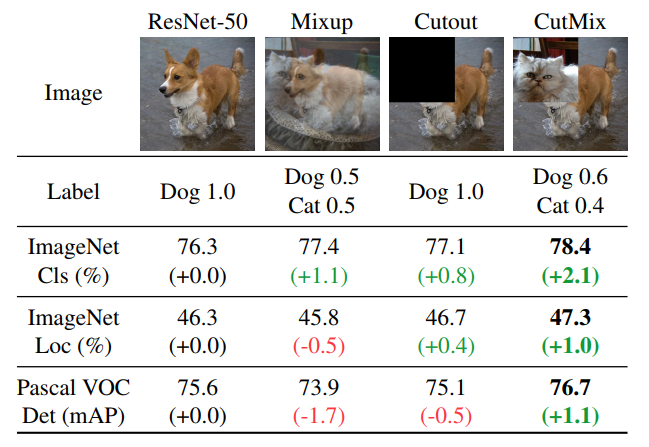
\includegraphics[width=0.5\linewidth]{pic/cutmix.png}
            % \caption{Caption}
            \label{fig:cutmix}
        \end{figure}
        \item Surprisingly they remain ineffective when training adversarially robust networks. 
        \item In this work, we revisit these common augmentation techniques.
    \end{itemize}
\end{frame}

